\documentclass[11pt,a4paper]{article}
%\documentclass[11pt,twoside, journal]{IEEEtran}

%\documentclass[11pt, twocolumn]{article}
%\pagestyle{plain}
%for Latex=>PS=>pdf!
\usepackage[dvips]{graphicx}
\usepackage{psfrag}


\begin{document}

\pagestyle{empty}

\begin{figure}
\psfrag{A1}[c][c]{\large{Analysis I (1950/55)}}
\psfrag{A2}[c][c]{\large{Analysis II (1980/85)}}
\psfrag{A3}[c][c]{\large{Analysis III (2010/15)}}
\psfrag{C11}[l][l]{\small{Cluster 1/I}}
\psfrag{C21}[l][l]{\small{Cluster 2/I}}
\psfrag{C31}[l][l]{\small{Cluster 3/I}}

\psfrag{C12}[l][l]{\small{Cluster 1/II}}
\psfrag{C22}[l][l]{\small{Cluster 2/II}}
\psfrag{C32}[l][l]{\small{Cluster 3/II}}

\psfrag{C13}[l][l]{\small{Cluster 1/III}}
\psfrag{C23}[l][l]{\small{Cluster 2/III}}
\psfrag{C33}[l][l]{\small{Cluster 3/III}}
\includegraphics[]{map1.eps}
\includegraphics[]{map2.eps}
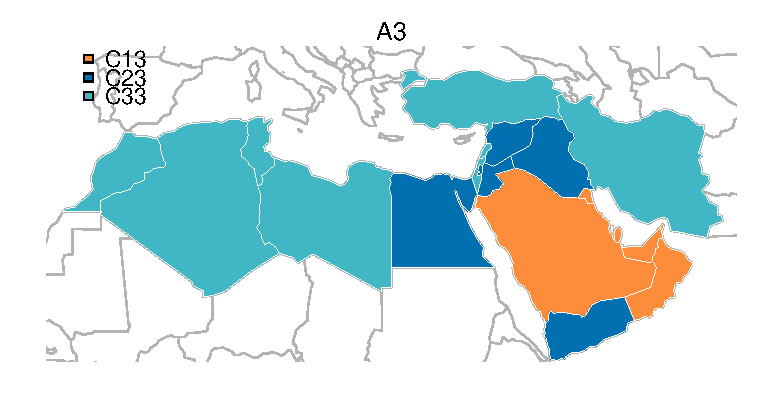
\includegraphics[]{map3.eps}

\caption{Mapping the three different cluster analyses}
\end{figure}




\end{document}